To build intuition for the two models,
Figure \ref{fig:numerical} shows a numerical
simulation of data from a HMM model,
and the results for the HMM model,
in panel A, and the
two-step model, in panel B.
Whereas the HMM model's posterior predictions
switch from body to tail depending on
the particular latent state path,
the two-step models have fixed
$\tau = 6$ and $\rho_{1,2} = (6, 10)$.
As shown by the ELPD values above each
plot, the HMM variant outperforms
the two-step approach for all
experience periods except the first,
where our chosen value $\tau$
matches the HMM data-generating process
exactly. In other experience
periods, the two-step approach
generalises poorly. This illustrates that,
if $\tau$ is chosen correctly, and the
tail model is trained on suitable development
lags, the two-step approach can provide
more exact predictions, because
uncertainty in the latent state
from the HMM model hurts predictive accuracy.
However, if
experience periods differ in their
body-to-tail switch-over dynamics,
which is expected, then overall
performance suffers due to
growing generalisation error.

\begin{figure}
    \hspace{-1.8cm}
    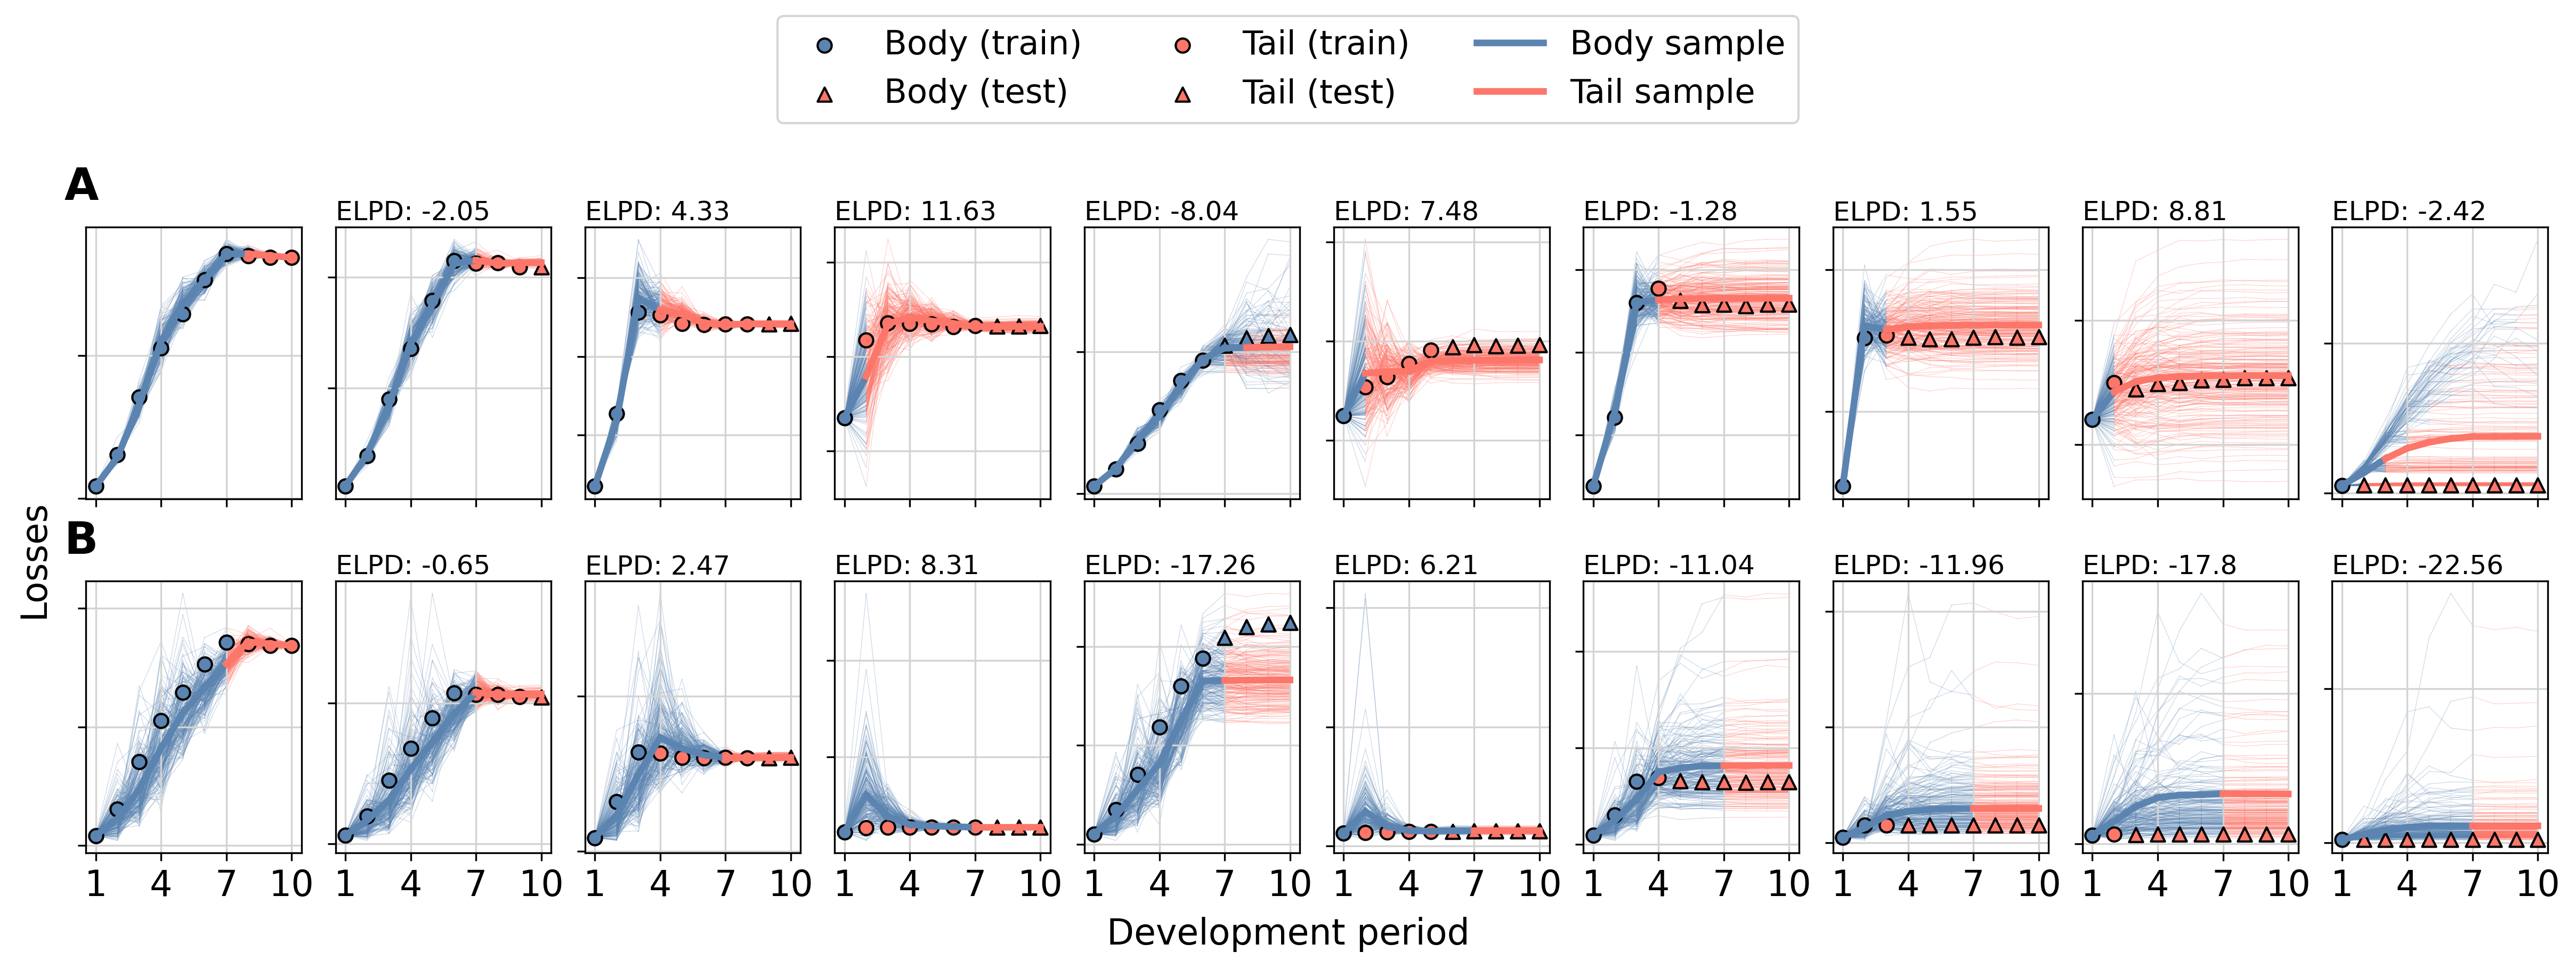
\includegraphics[scale=0.45]{\figures/numerical}
    \caption{
        A simulated data example comparing the HMM
        to two-step process to build intuition.
        Panels A (HMM) and B (two-step) show
        10 experience periods from a single
        loss triangle simulated from the HMM
        model. The true losses
        are shown as points, with colours
        identifying
        body (blue) or tail (orange) points.
        Circles denote training data and
        triangles test data. Thin 
        lines are samples from the posterior
        predictive distributions, coloured
        by latent state, and the thicker
        line shows the mean paths.
        The ELPDs on the test data
        points in each experience period
        are shown above each plot.
        The two-step model was fit
        assuming $\tau = 6$ and
        $\rho_{1,2} = (6, 10)$.
    }
	\label{fig:numerical}
\end{figure}

Simulation-based calibration of the HMM model indicated
no problems with model calibration (Figure \ref{fig:sbc}),
with all histograms matching the assumptions of
uniformity. However, 10 models were removed for poor
convergence, which typically occurred when the simulated
link ratios from the body process were
higher than values expected from real loss triangles. 
Given this occurred rarely, the priors were left
unchanged, although suitable prior distributions
for Bayesian chain ladder models is an area
with a dearth of literature.
For the 990 models, 
the average classification accuracy of the recovered latent
state values $\bm{z}$, across
both training and test data, was 97\% with a 
95\% highest density interval (i.e. the 95\% most
likely values) of [91, 100].

\begin{figure}
    \centering
    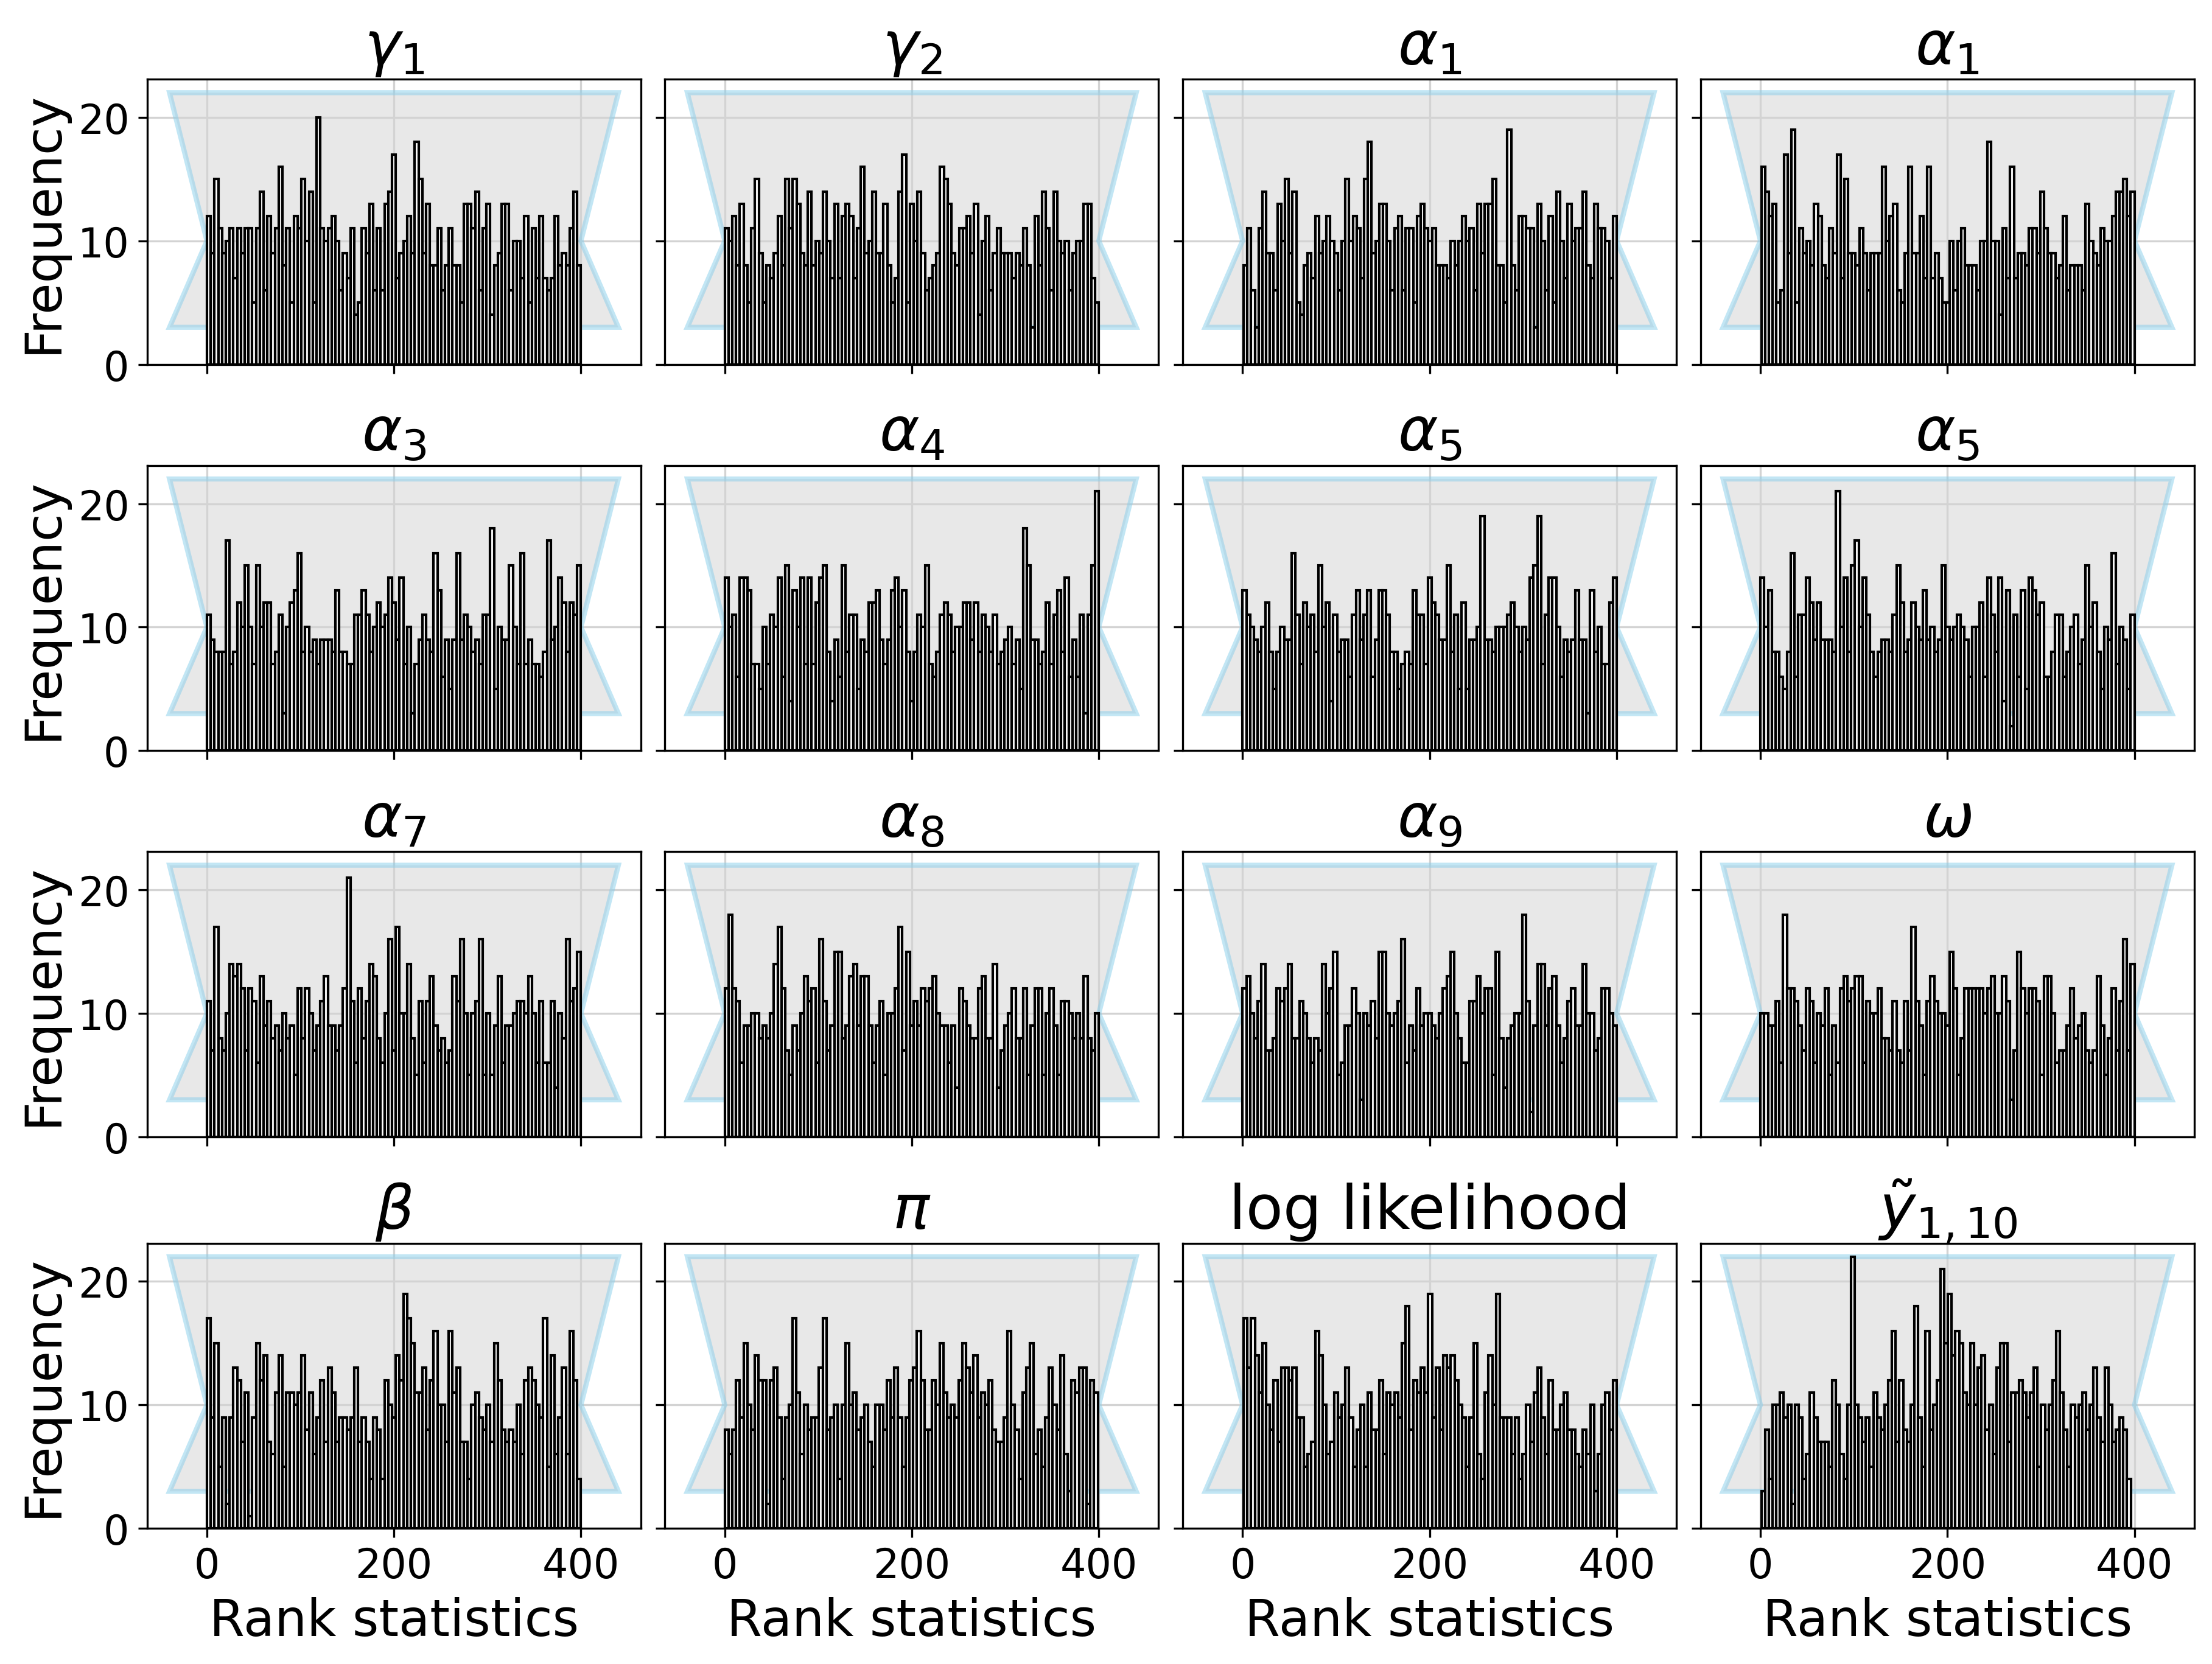
\includegraphics[scale=0.5]{\figures/ranks}
    \caption{
		Histograms of simulation-based calibration
		rank statistics for the HMM model, 
        with the 99\% percentile
        interval from a discrete uniform distribution
        shown in the grey shaded band.
        Each histogram shows a key model parameter,
        and the final two panels show the ranks
        for the joint log
        likelihood and the first ultimate loss
        distribution.
        For each model, we sampled
        4000 draws from the posterior distribution,
        and thinned the samples by 10 to remove any
        autocorrelation, meaning a maxmimum rank statistic
        of 400. Of the 1000 models,
        10 were removed due to poor convergence.
    }
	\label{fig:sbc}
\end{figure}

The ELPD and RMSE differences between models (compared to the
HMM base model) are shown in Figure \ref{fig:backtest-scores}.
When calculating ELPD, a small number of pointwise log densities 
showed very small, negative values, indicating poor predictions
on the out-of-sample data leading to numerical instability. 
We decided to remove any log predictive
densities for all models that had values $< -100$, which for a single
out-of-sample data point was particularly low, given that most
ELPD values for a single data point lie within [-5, 5]. This retained 99.91\%
of values for the PP results, 99.42\% of values for WC, 99.64\%
for CA, and 98.38\% for OO. The full log densities are given in the
supplementary materials, as well as results for different levels
of filtering.

For ELPD and RMSE, at least one of the
hidden Markov model variants out-performed
the two-step approach, apart from ELPD
for PP and WC lines of business, where
a small proportion of the
two standard errors 
included zero (Figure \ref{fig:literature}).
Overall, the HMM-$\nu$ model attained
75\% of the best average ELPD scores, and 50\%
of the best average RMSE scores, meaning that
allowing for tail processes to revert
to the body is important to making
future predictions.
Evaluating the predictions at the lag-10
out-of-sample values only, to mirror
the estimation of ultimate loss,
mirrored the results in Figure
\ref{fig:backtest-scores} apart from some
minor changes in ranks of the HMM
models (full results supplied
in the supplementary materials).

\begin{figure}
    \centering
    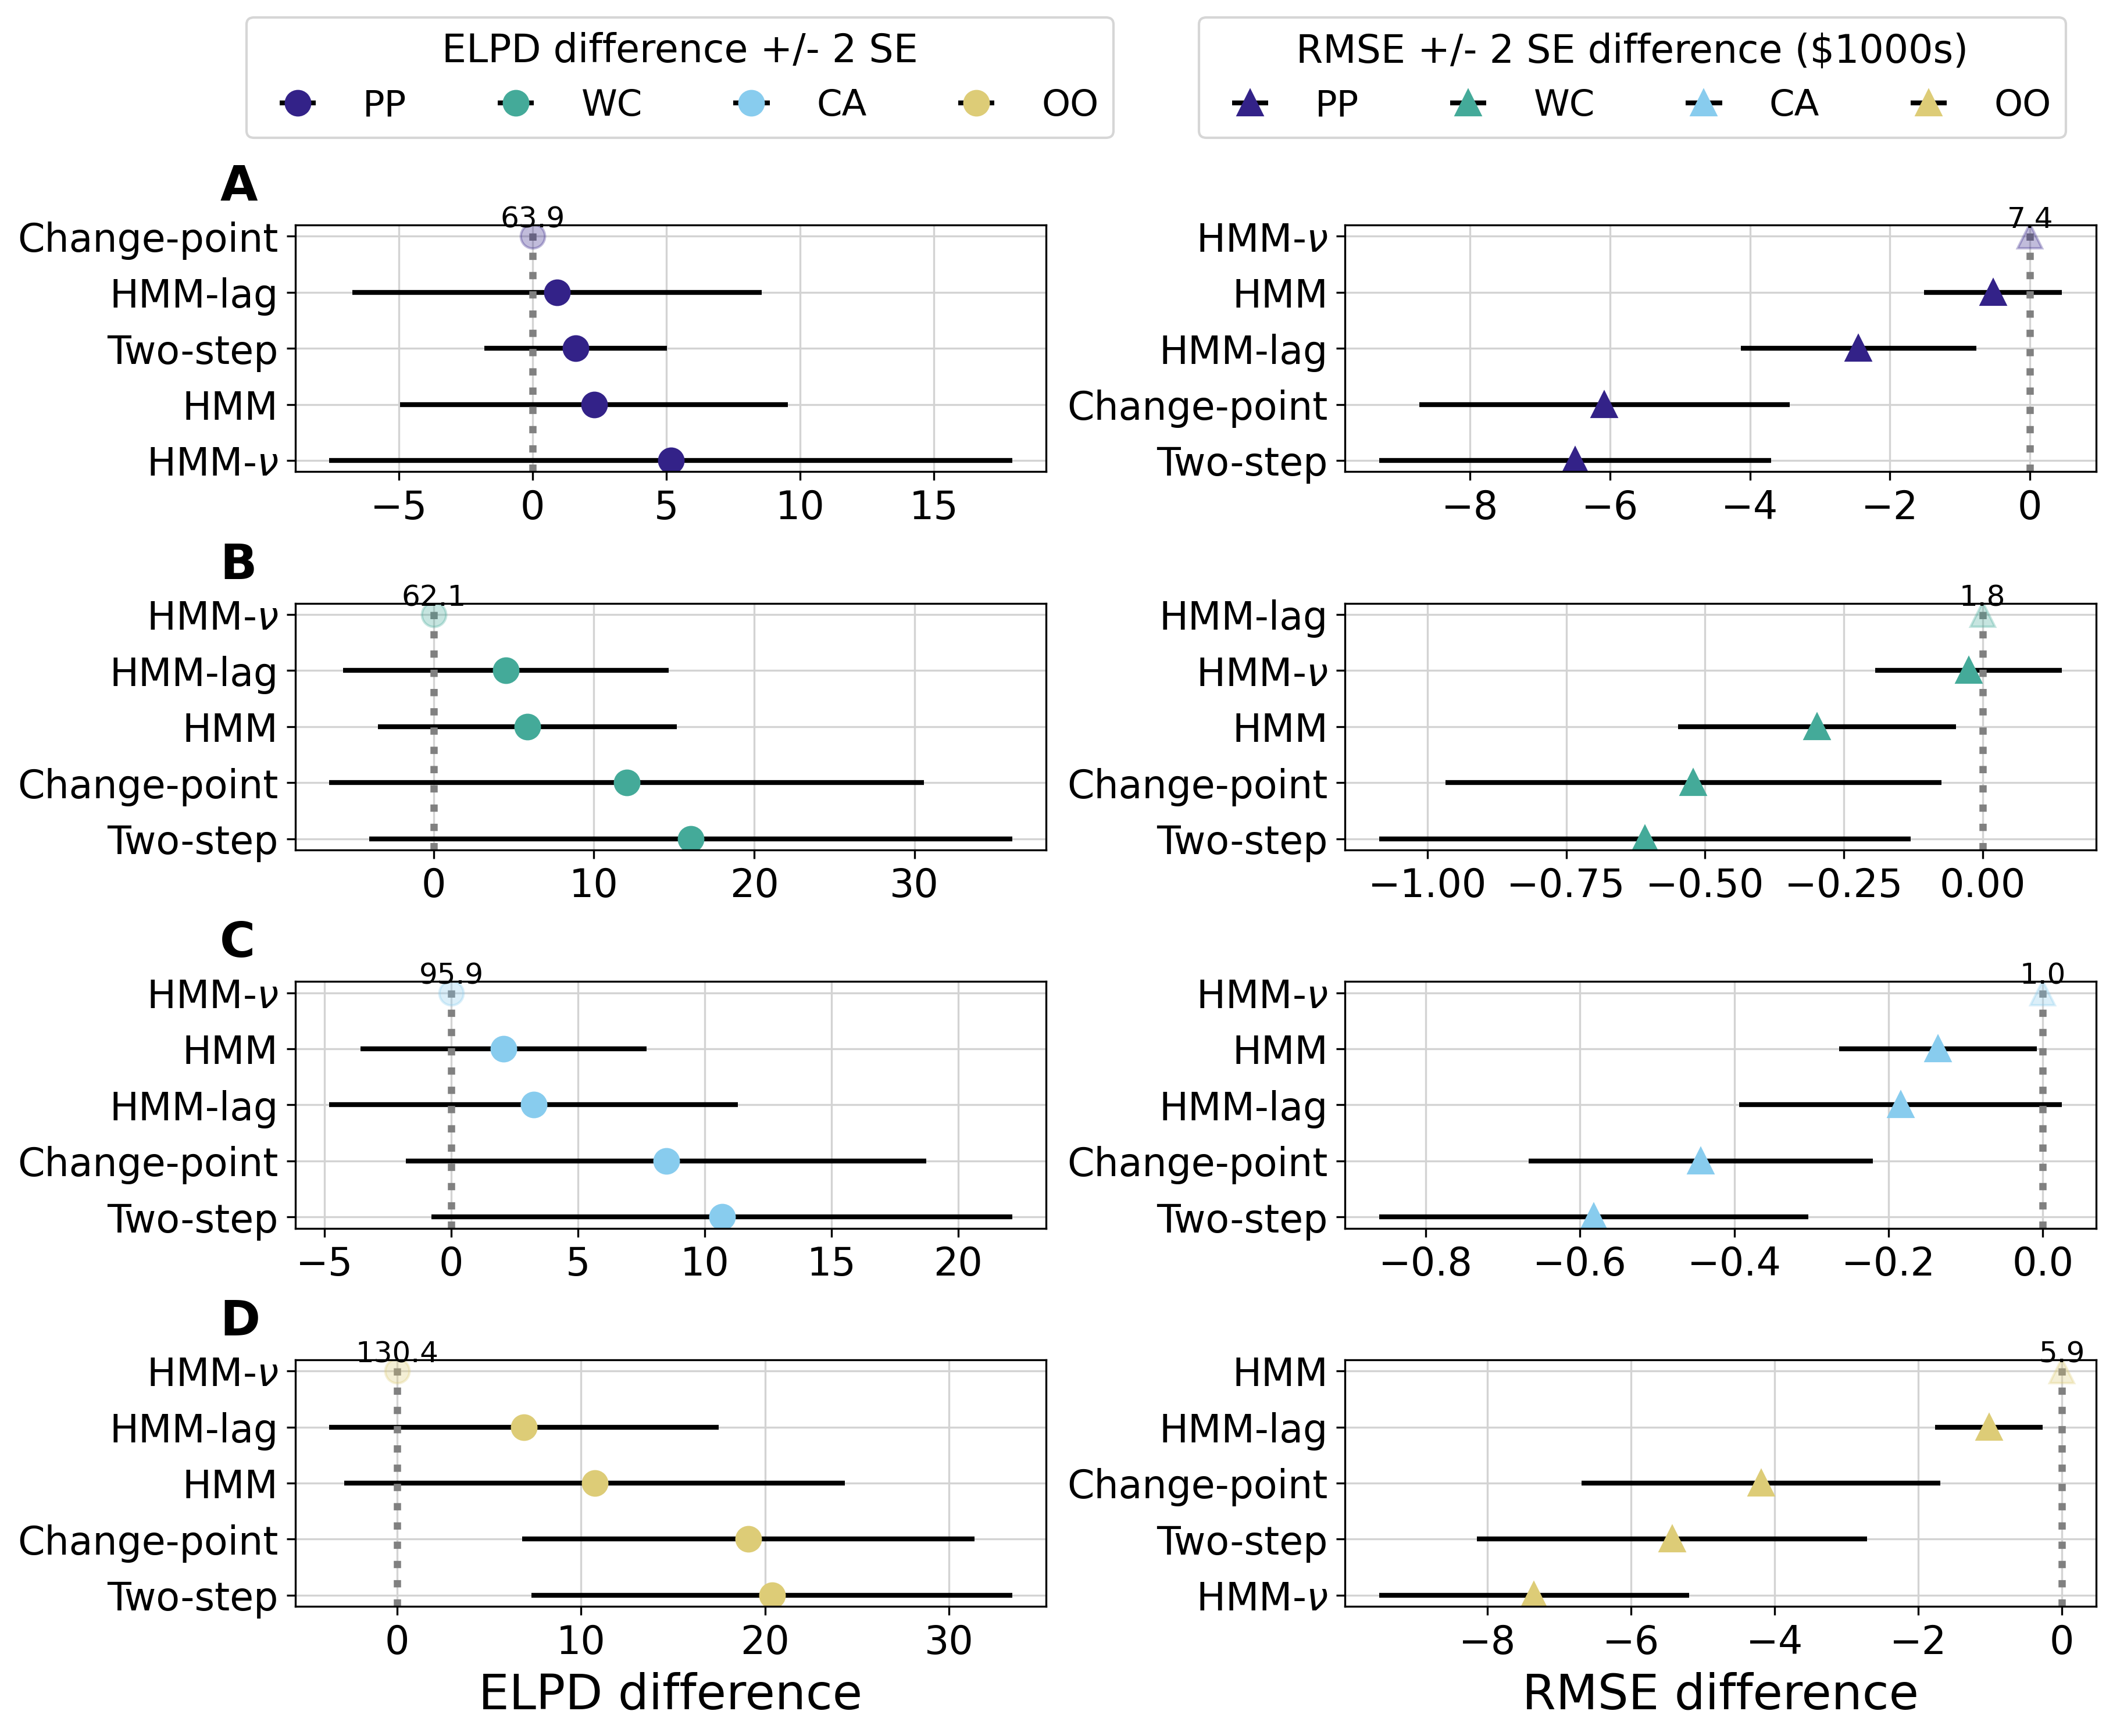
\includegraphics[scale=0.5]{\figures/scores.png}
    \caption{
        The ELPD (left column) and RMSE (in thousands of dollars; right column)
		differences (+/- 2 standard errors; SE) in order of performance
        for each model and line of business for the industry
        triangles. Rows A through D enumerate results
        for line of business separately.
        The best-performing model is shown at the top of each
        panel, with the absolute ELPD or RMSE value displayed above.
        Positive ELPD differences with an uncertainty interval that does not
        cross zero indicates a credible difference at the 95\% level
        in favour of the top model.
        Negative RMSE differences with an uncertainty interval
        that does not cross zero indicates a credible difference
        in favour of the top model.
    }
	\label{fig:backtest-scores}
\end{figure}

Model calibration histograms (Figure \ref{fig:percentiles})
indicated that both the hidden Markov models
and two-step approaches typically have predictions that
are too uncertain, indicated by the inverted-U shaped
histograms. In WC, the hidden Markov models had the most
uniform percentiles, whereas the two-step approach
showed signs of both under- and over-estimation.

\begin{figure}
    \centering
    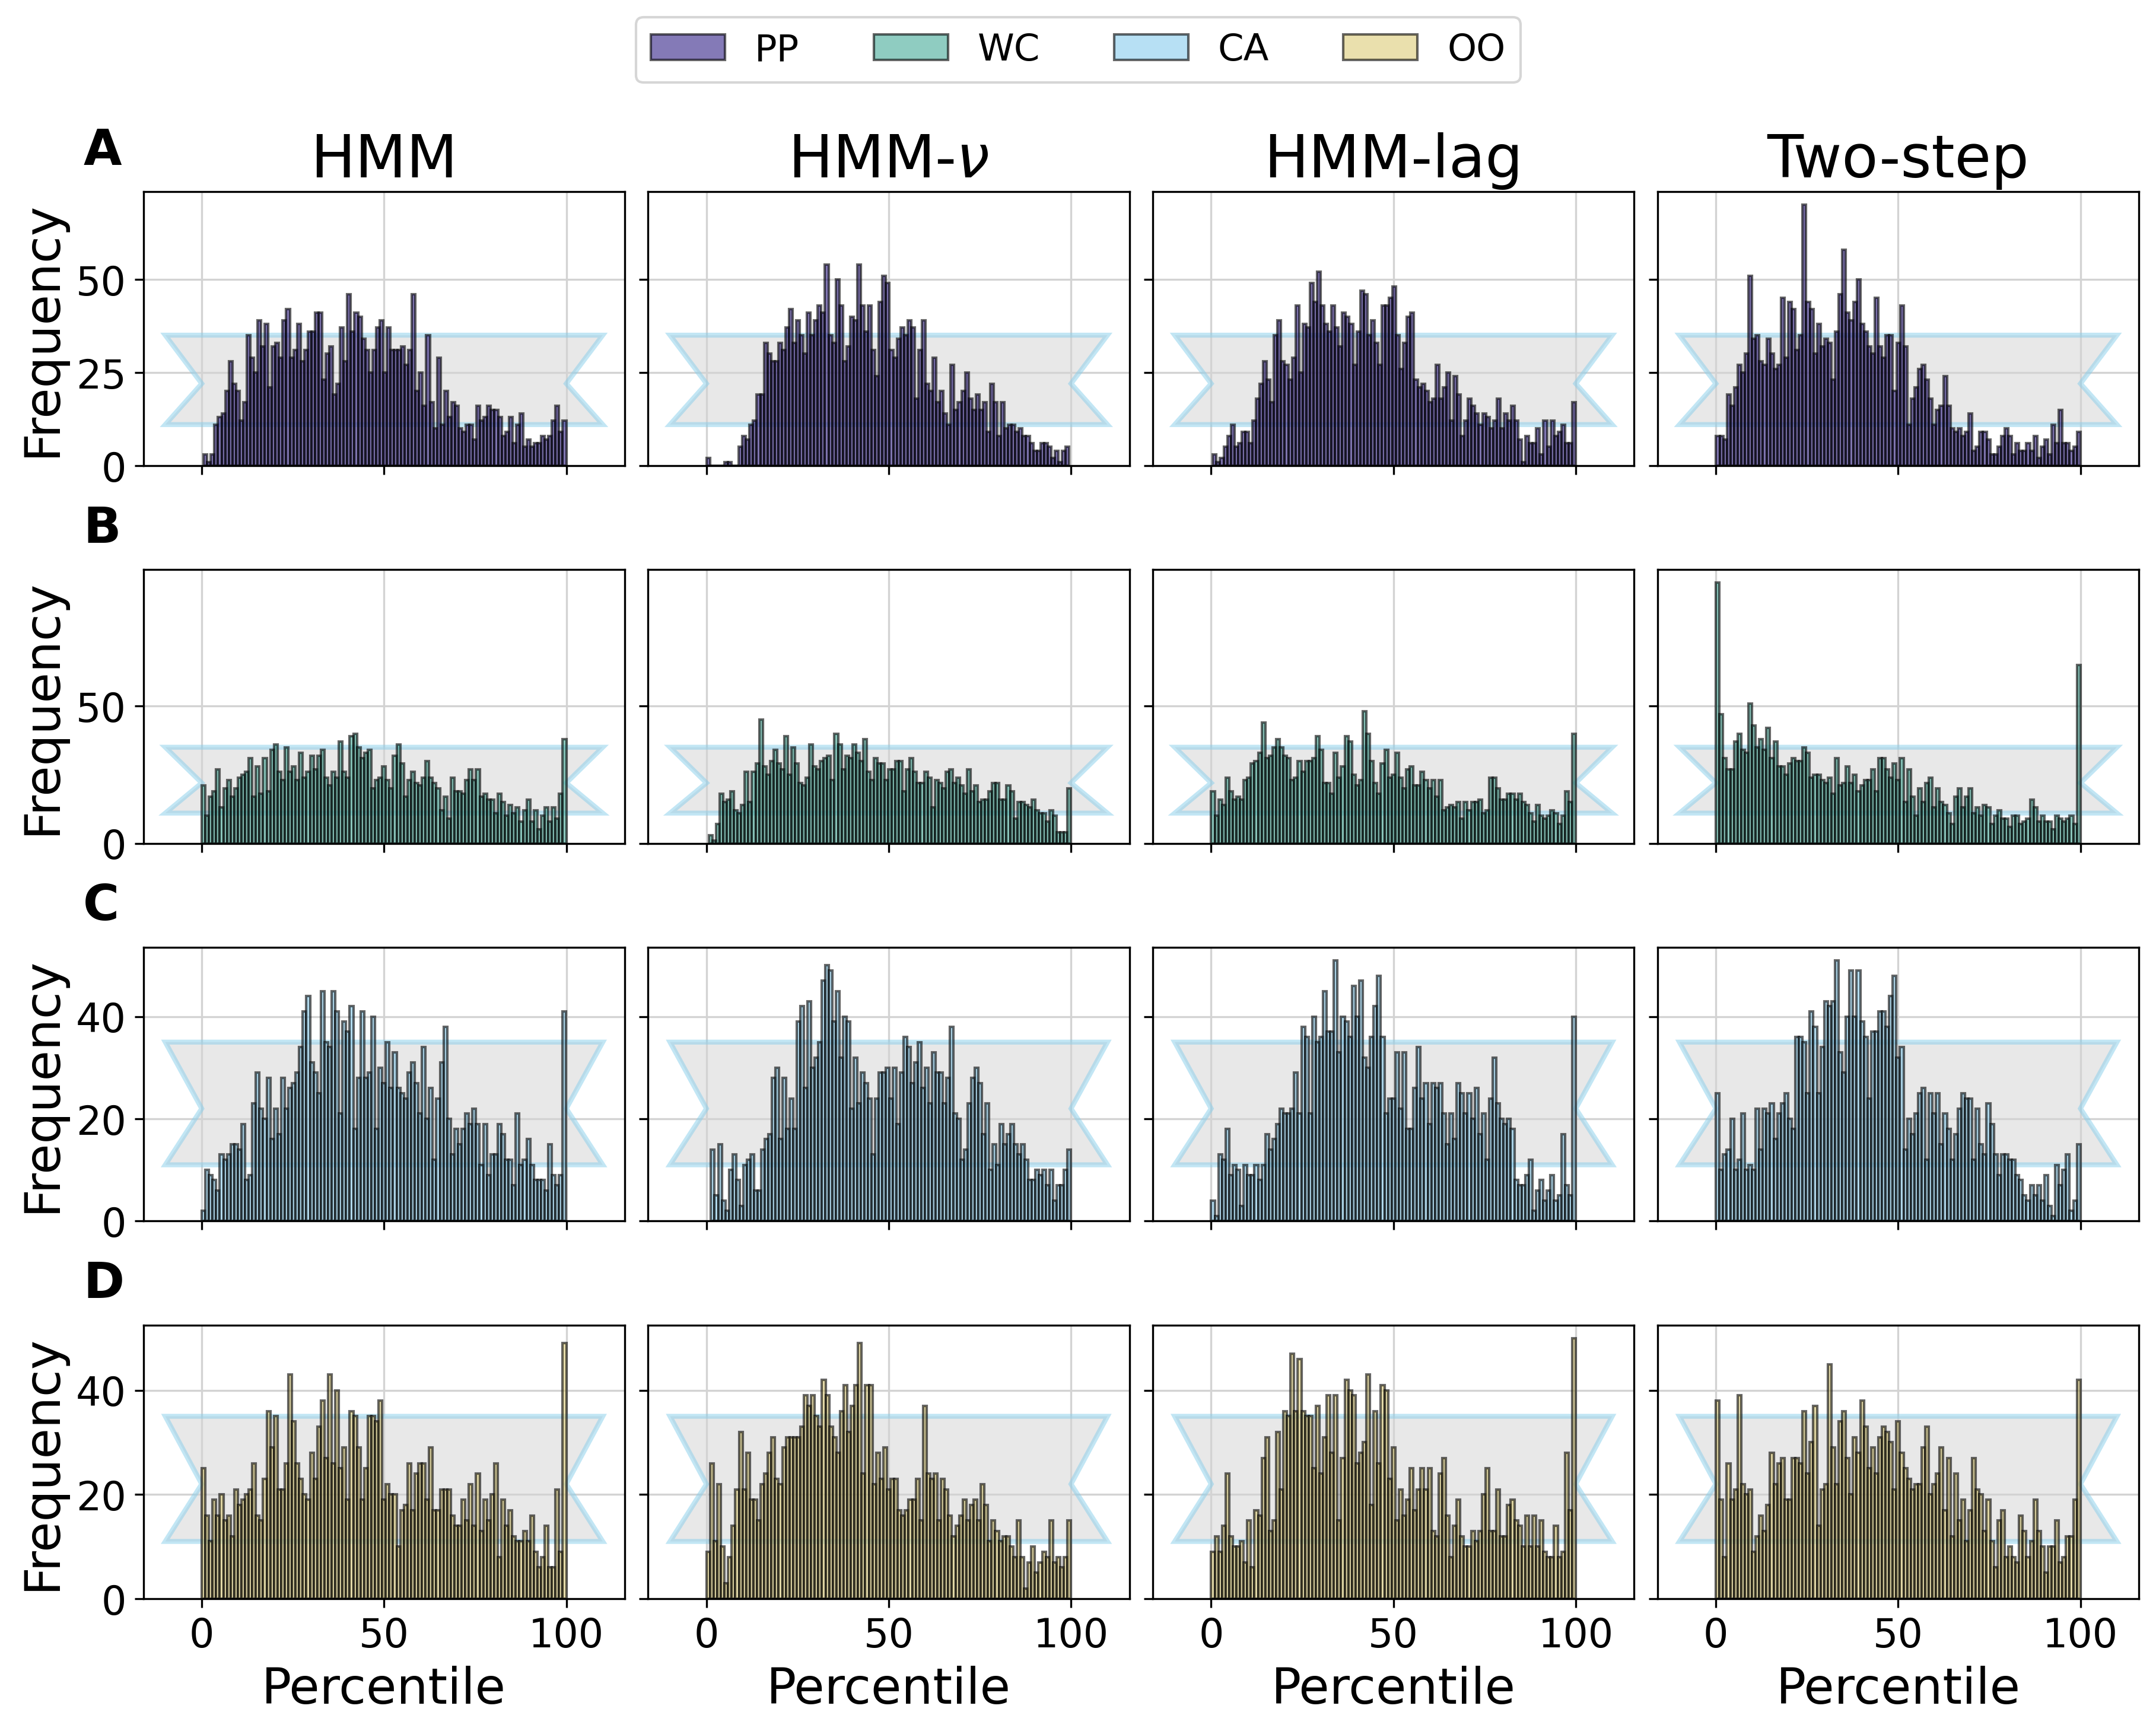
\includegraphics[scale=0.5]{\figures/calibration.png}
    \caption{
        Percentiles of the true left-out values on the posterior distributions
        for each model and line of business (panels A through D) in the industry triangles.
        Grey shaded regions provide the 99\% intervals of a discrete uniform
        distribution, for reference.
        Right-skewed histograms indicate under-estimation,
        left-skewed histograms indicate over-estimation,
        and inverted-U histograms indicate predictions that
        are uncertain.
    }
    \label{fig:percentiles}
\end{figure}

The hidden Markov model variants had different
implications for body-to-tail switch-over points
depending on the particular line of business
(Figure \ref{fig:zstars}).
The PP and CA lines showed, in general,
the quickest development to the tail
state, at development lag 2 for the HMM
and HMM-$\nu$ models, and by development
lag 3 for most accident periods for the
HMM-lag model. In contrast, WC stayed
longest in the body state, followed by
OO, and both WC and OO lines demonstrated
relatively equitable probabilities of being
in the body and tail at later development
periods. This is particularly noticeable for
the HMM-$\nu$ model, where the chance
of returning to the body from tail process
was allowed.

\begin{figure}
    \centering
    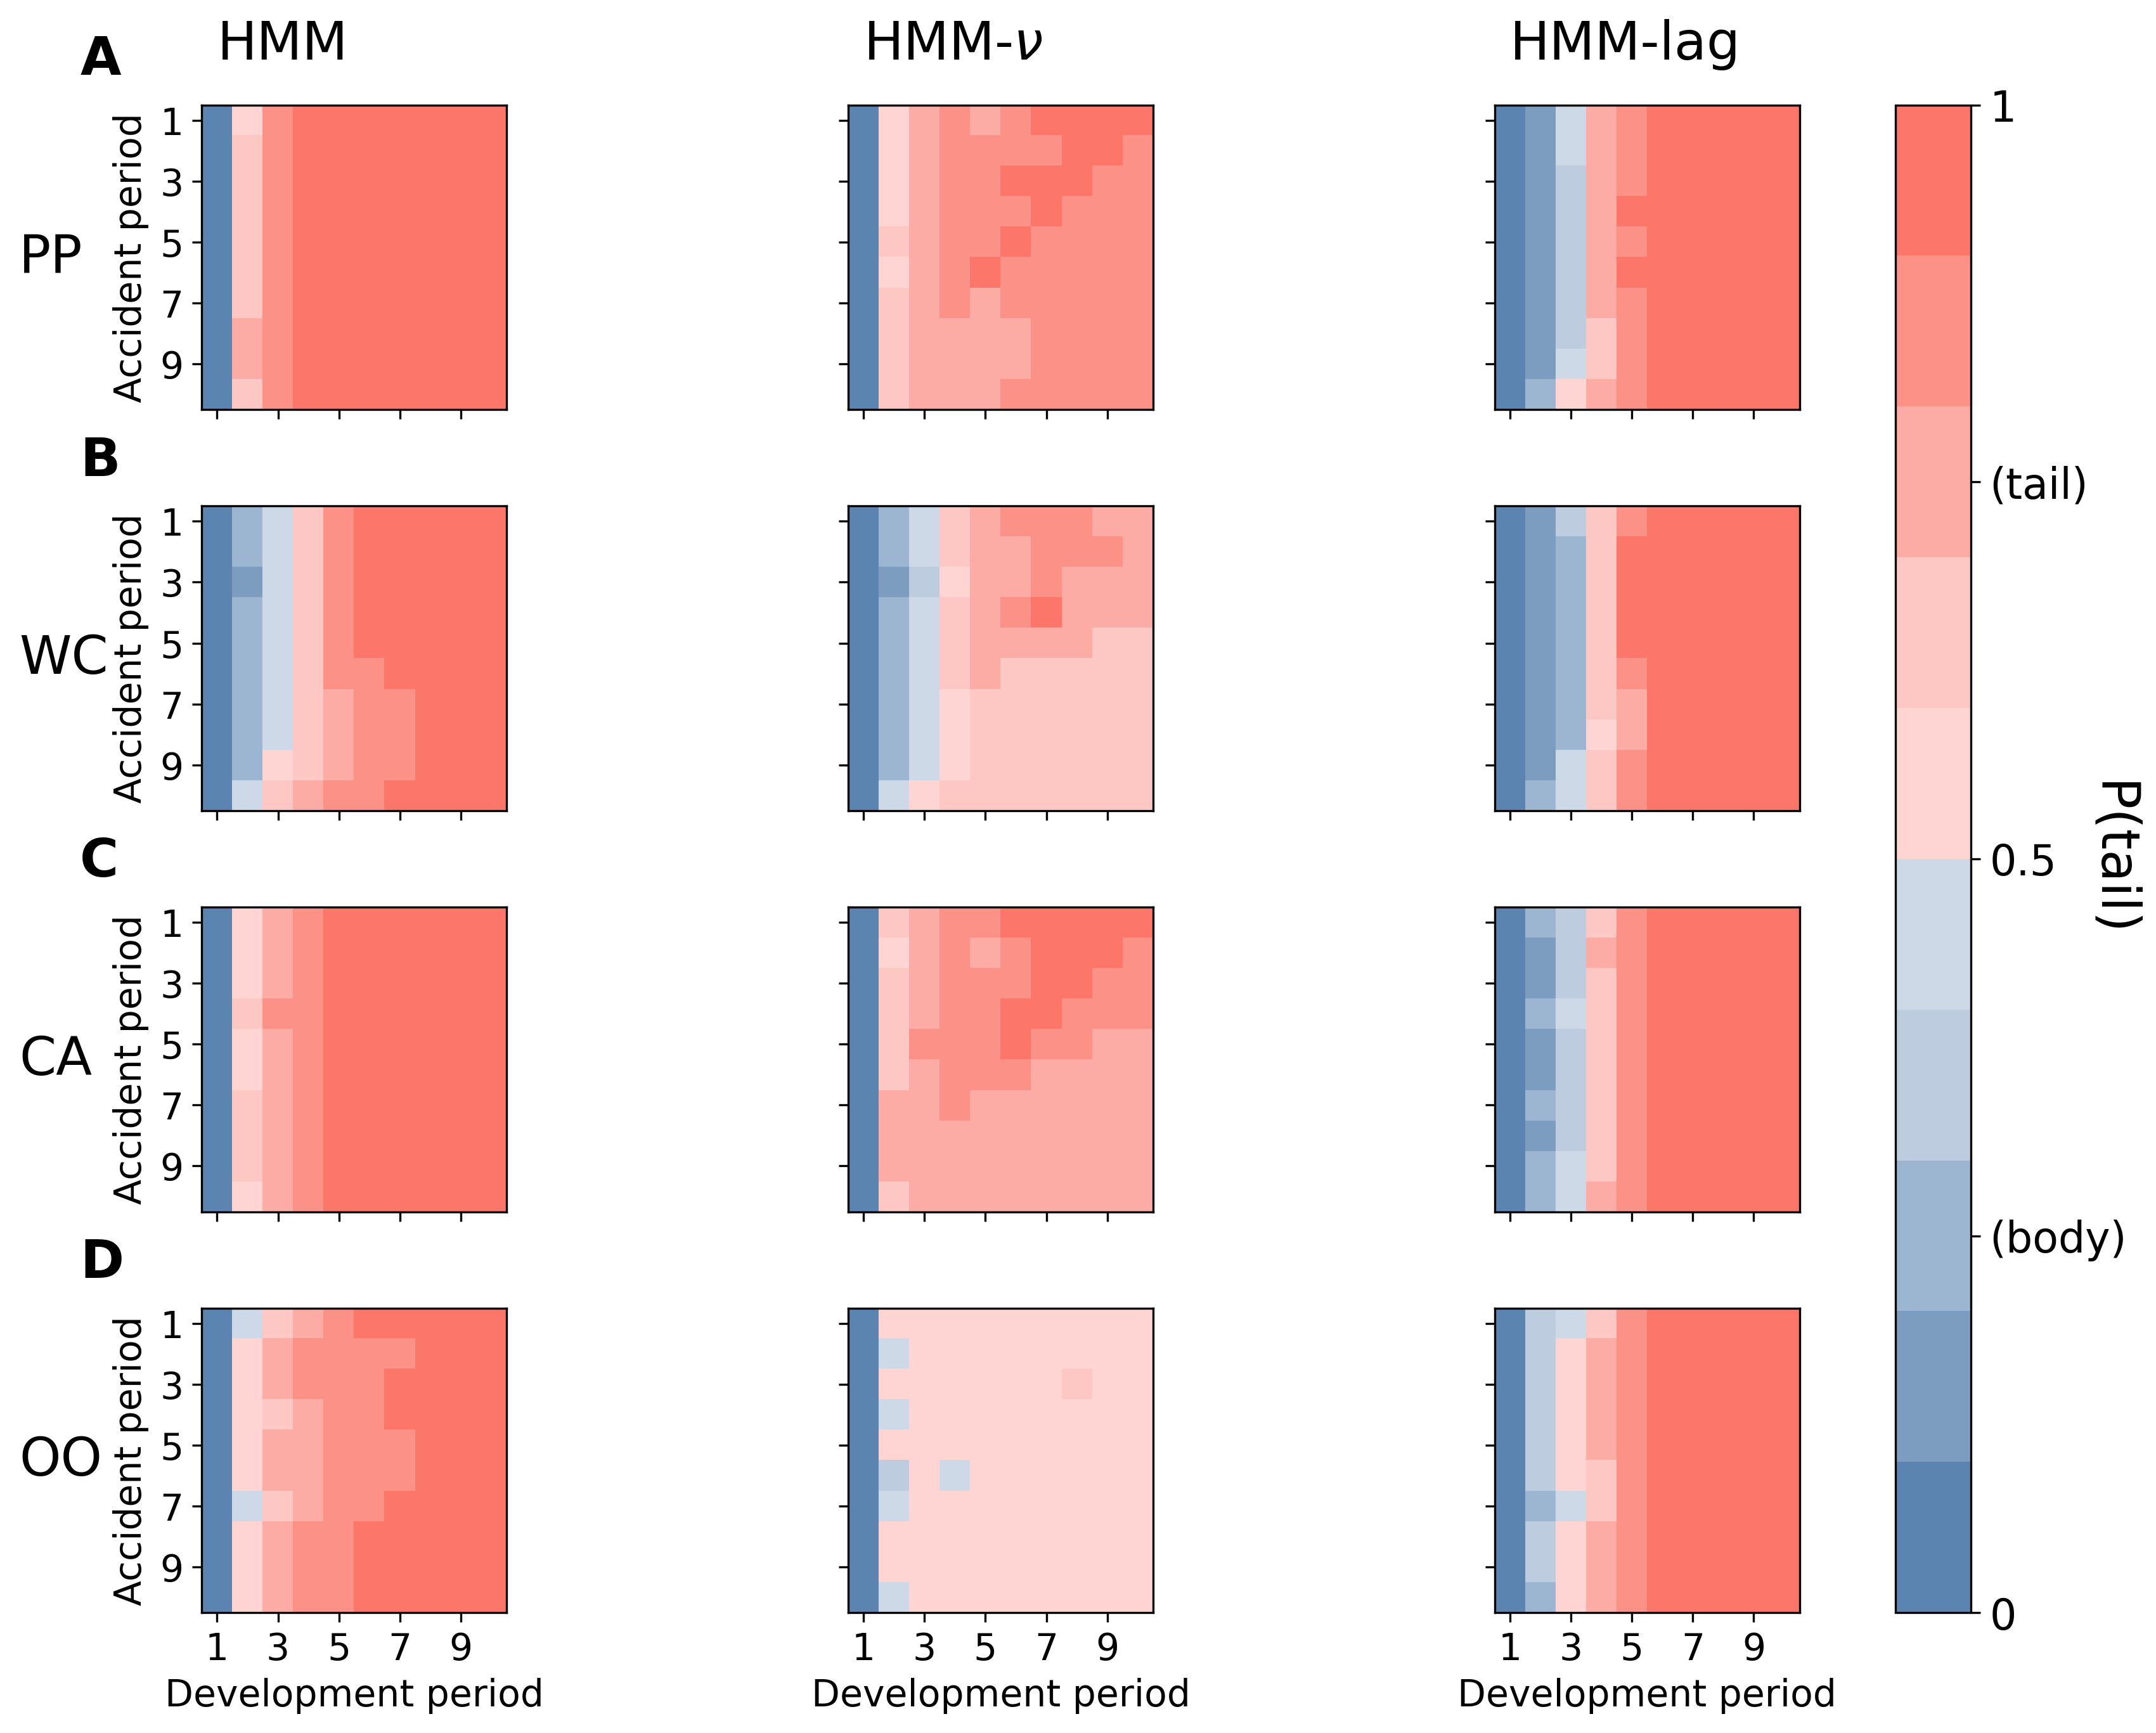
\includegraphics[scale=0.5]{\figures/z_stars.png}
    \caption{
        The average probability of being in the tail process
        for each hidden Markov model parameterization (columns)
        and line of business (rows A-D) across triangles
        in the industry data.
        Probabilities $\leq 0.5$ are coloured
        in blue whereas probabilities $> 0.5$
        are coloured in orange. More faded squares
        indicating smaller probabilities of being
        in body and tail processes, respectively.
    }
    \label{fig:zstars}
\end{figure}

For the five literature triangles, the lack
of hold-out data meant that the uncertainties
around the ELPD and RMSE differences
indicated more equal model performance
(Figure \ref{fig:literature}).
The average ELPD and RMSE
differences indicated that one of the hidden
Markov models often performed better than the
two-step approaches. The two-step approach
out-performed the hidden Markov models
for the \cite{merz2015} triangle,
and ranked second for RMSE
for three of the five triangles.
The manual selection of $\tau$
for the two-step process often
closely aligned with the 
development lag from the
best-performing HMM where
the probability of being in
the tail was $> 0.5$. The one
exception was
the long-tailed
liability triangle of
\cite{balona2022},
where the chosen $\tau$
of 12 was much larger
than the most likely
switch-over lag from the HMM
variant of $j=3$. However,
$j=3$ did closely match
the choice of $\rho_{1} = 4$.

\begin{figure}
    \centering
    \hspace{-1em}
    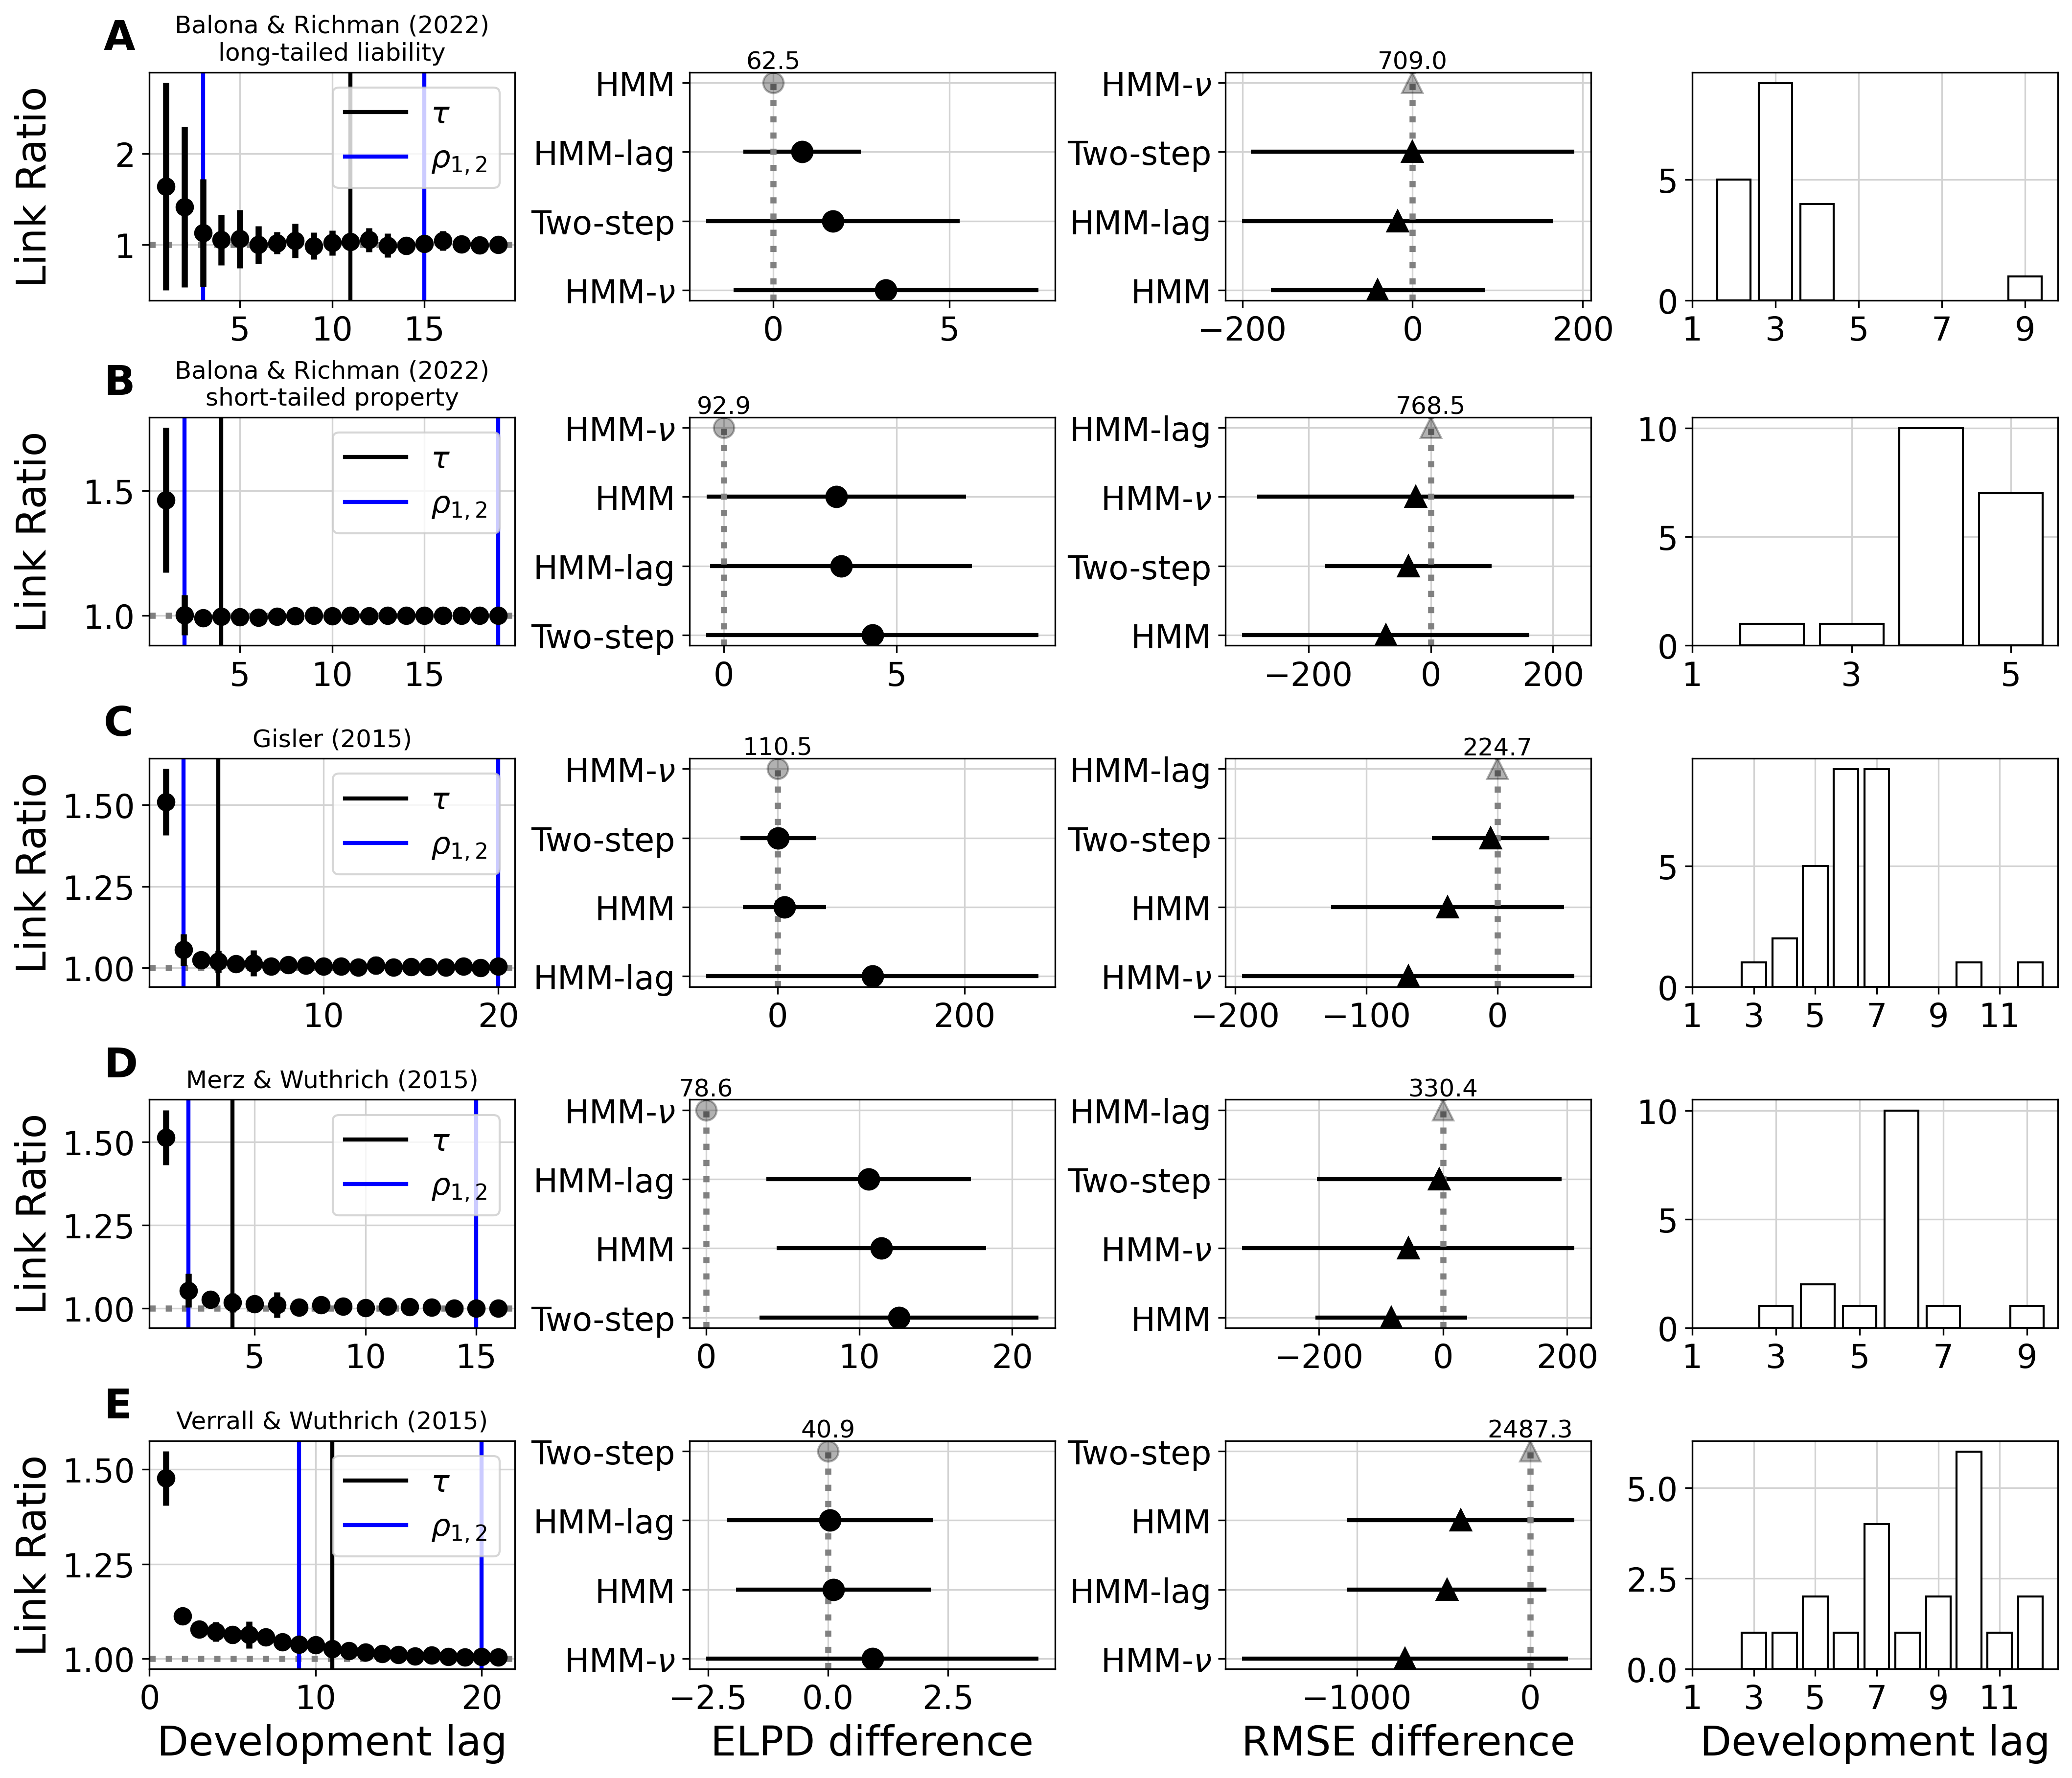
\includegraphics[scale=0.45]{\figures/literature.png}
    \caption{
        Results for the hidden Markov model and two-step
        approach on the five literature triangles
        (rows A - D). The first
        column shows the mean (+/- 2 standard deviations)
        of the empirical link ratios in the triangles.
        The black and blue vertical lines indicate $\tau$
        and $\bm{\rho} = \rho_{1:2}$, the tail start
        and generalised Bondy model training windows,
        respectively (see model definitions, above).
        The second and third columns show the
        ELPD and RMSE differences (+/- 2 SE) from the best
        performing model (top model in each panel), calculated
        from predictions on the latest diagonal of
        data (out-of-sample) in the loss triangles.
        The absolute ELPD and RMSE of the best-performing
        models are shown above the top model, for reference.
        The final column shows the development lags where
        the probability of being in the tail was $> 0.5$
        for the highest ELPD hidden Markov model
        variant.
    }
	\label{fig:literature}
\end{figure}

